\chapter{GENETIC REGULATION OF MOSQUITO DEVELOPMENT}
\section{Introduction}

The development of mosquitoes requires the precise involvement of a variety of different genes. These genes each serve a unique function that must be appropriately timed to the correct stage of development. These genes can be involved in many different processes, such as feeding, hormone production, tissue development, circadian rhythm, and immunity \citep{smith2004}. 

\section{Gene ABC}

Gene ABC is one of many genes involved in the regulation of mosquito development. Gene ABC codes for the protein, Protein ABC (see Fig. \ref{fig:protein}). 

\begin{figure}[b!]
	\centering
	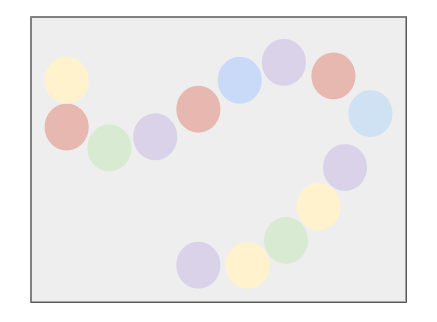
\includegraphics[width=0.8\linewidth]{Images/protein.png}
	\caption{Diagram of Protein ABC}
        \label{fig:protein}
\end{figure}


\subsection{Function of Gene ABC in Larval Stage}

Gene ABC drives many of the physiological processes necessary for successful larval development. It primarily plays a role in regulating the rate of larval feeding. It has also been shown to affect the release of several different hormones throughout larval development. These hormones have sweeping effects on subsequent development.

\subsubsection{Expression of Gene ABC in First Larval Instar}

The expression of Gene ABC is highest during the first four hours of the first larval instar stage. Expression then drops dramatically over the next four hours. The rate of expression then gradually increases until the end of the first instar stage. This pattern suggests a varied need for Protein ABC during development. 

\paragraph{Feeding Effects}
One of the primary behaviors regulated by Gene ABC is feeding. Larvae feed rigorously during the first four hours post-hatching. Feeding then drops off for the next four hours. Feeding gradually increases until the end of the first instar stage. This feeding pattern largely matches the expression of Gene ABC. 




